\chapter{Bijlages}
\label{ch:bijlages}

Om de leesbaarheid van de bachelorproef te behouden zijn sommige niet essentiële afbeeldingen, tabellen en overige documenten in dit hoofdstuk opgenomen. 

\section{Figuren literatuurstudie}
\label{sec:bijlages-literatuurstudie}

\FloatBarrier
\begin{figure}[h!]
	\centering
	\fbox{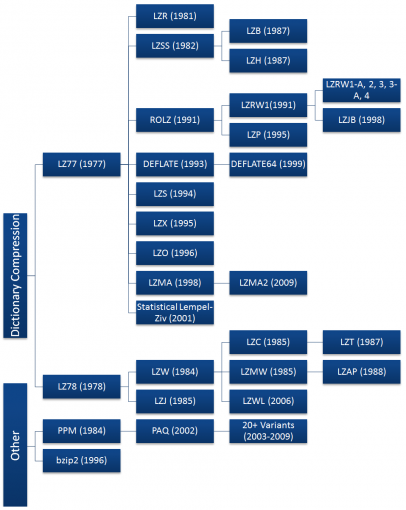
\includegraphics[width=0.45\linewidth]{img/literatuurstudie/lossles_datacompressie_overzicht.png}}
	\caption{Lossless datacompressie overzicht (\cite{ethwcompressionhistory})}
	\label{fig:lossles-datacompressie-overzicht}
\end{figure}
\FloatBarrier

\section{Screenshots datacompressietool}
\label{sec:bijlages-screenshot-datacompressietool}

De \gls{compressietool} is raadpleegbaar via de website van Lennert Bontinck\urlcite{compressietool}. De code is te vinden op de \gls{github} repository van deze bachelorproef\urlcite{githubbachelorproef}.

\FloatBarrier
\begin{figure}[h!]
	\fbox{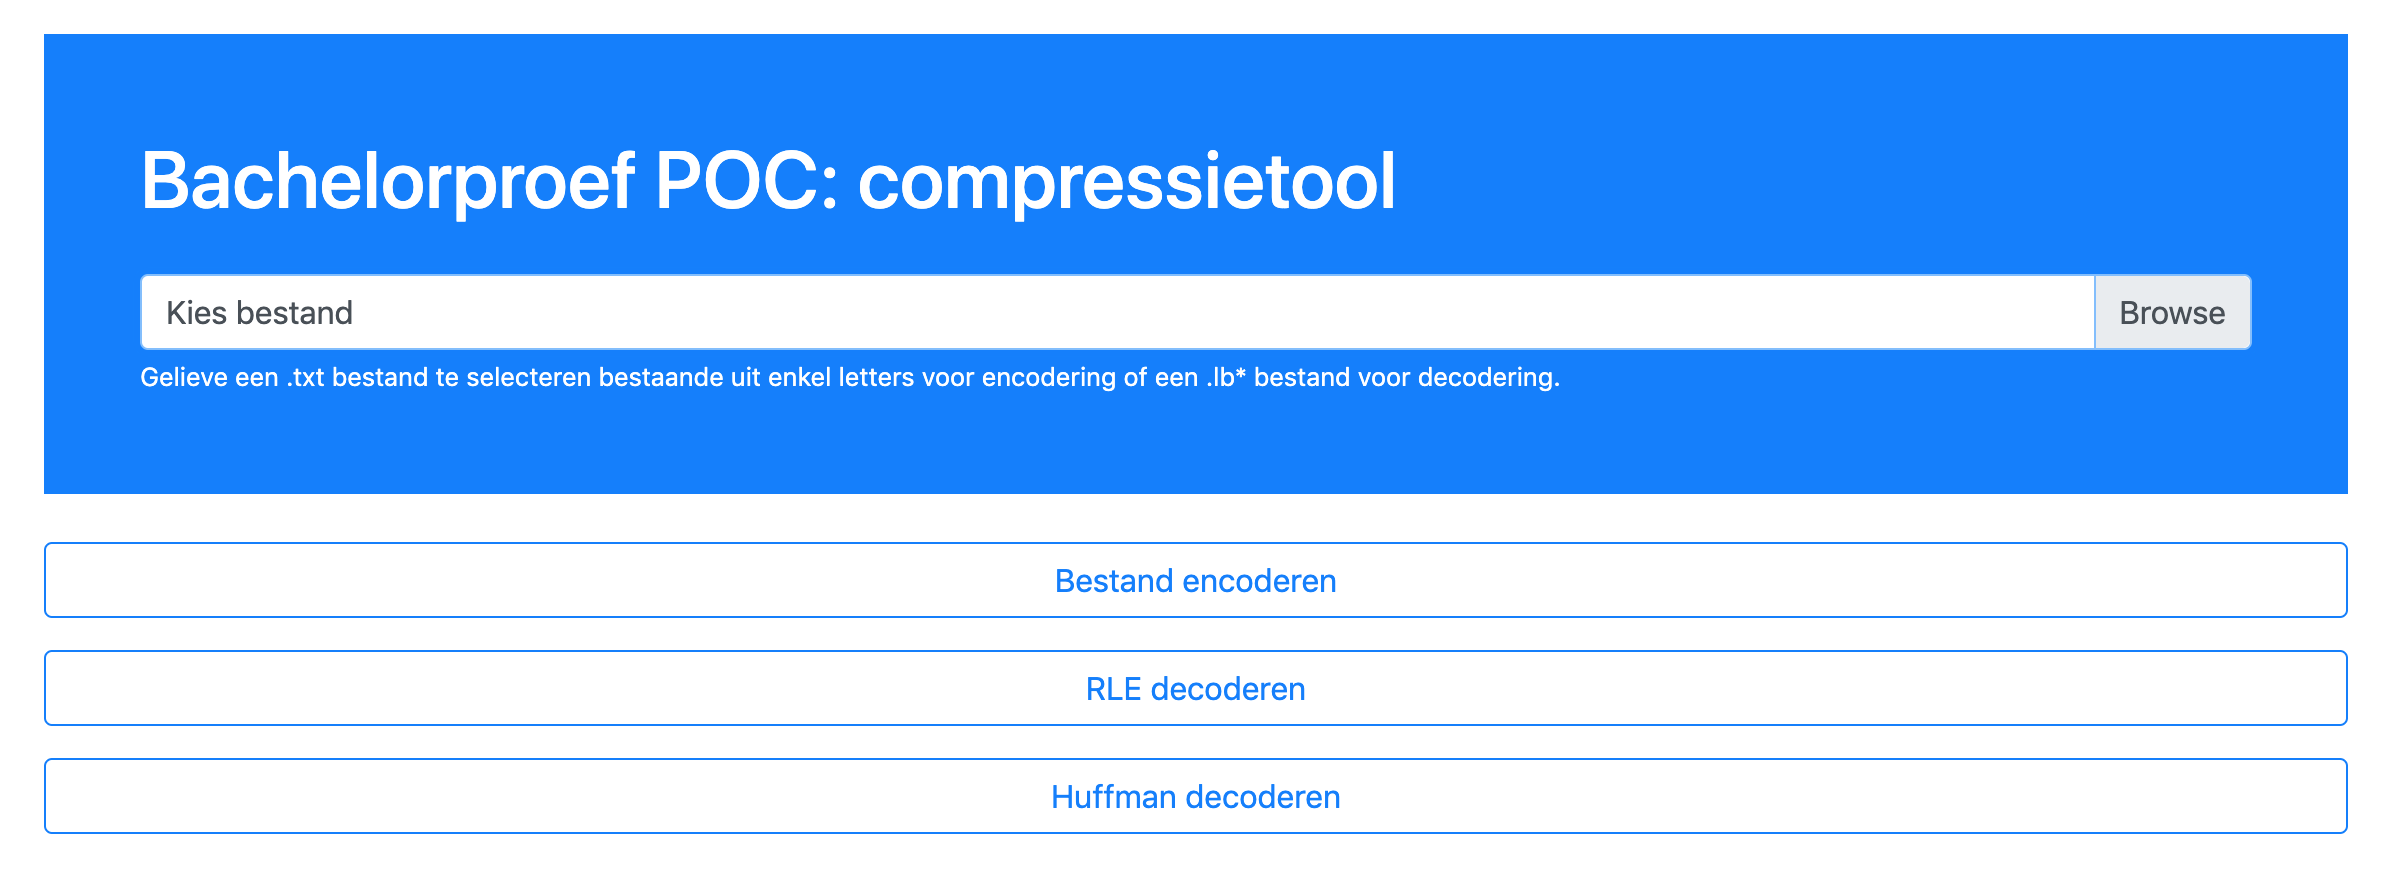
\includegraphics[width=\linewidth]{img/bijlages/compressietool/index.png}}
	\caption{Verwelkomingsscherm van de \gls{afbeeldingsevaluatietool}.}
	\label{fig:bijlages-screenshot-datacompressietool-index}
\end{figure}
\FloatBarrier

\FloatBarrier
\begin{figure}[h!]
	\fbox{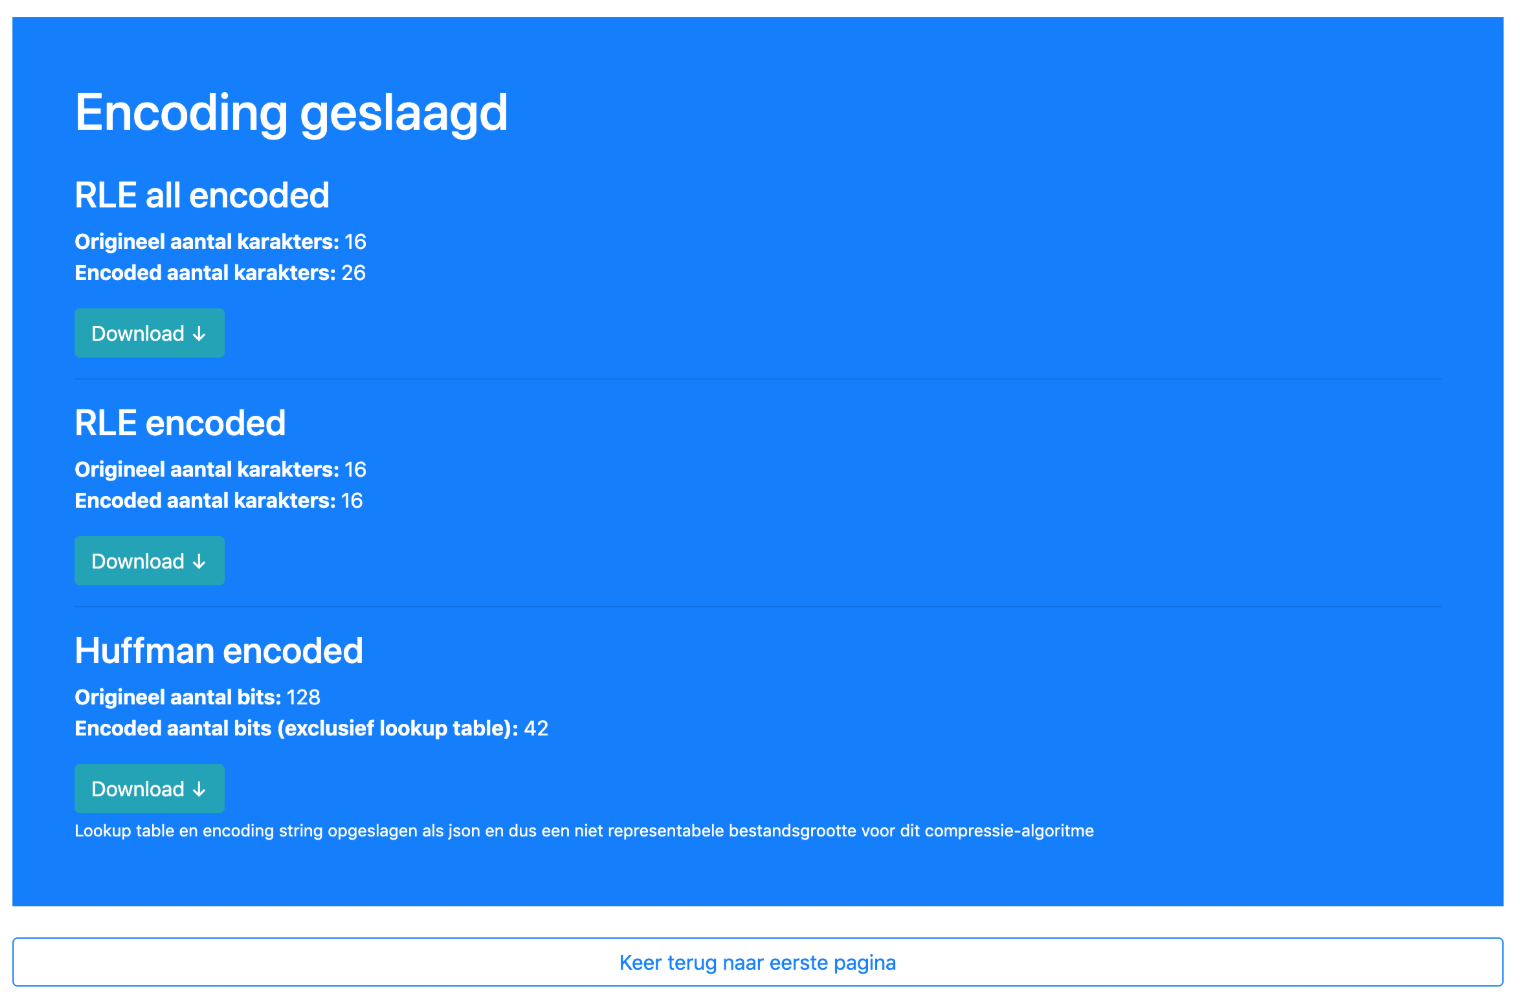
\includegraphics[width=\linewidth]{img/bijlages/compressietool/encoded.png}}
	\caption{Scherm verkregen door een bestand te encoderen \gls{afbeeldingsevaluatietool}.}
	\label{fig:bijlages-screenshot-datacompressietool-encoded}
\end{figure}
\FloatBarrier

\FloatBarrier
\begin{figure}[h!]
	\fbox{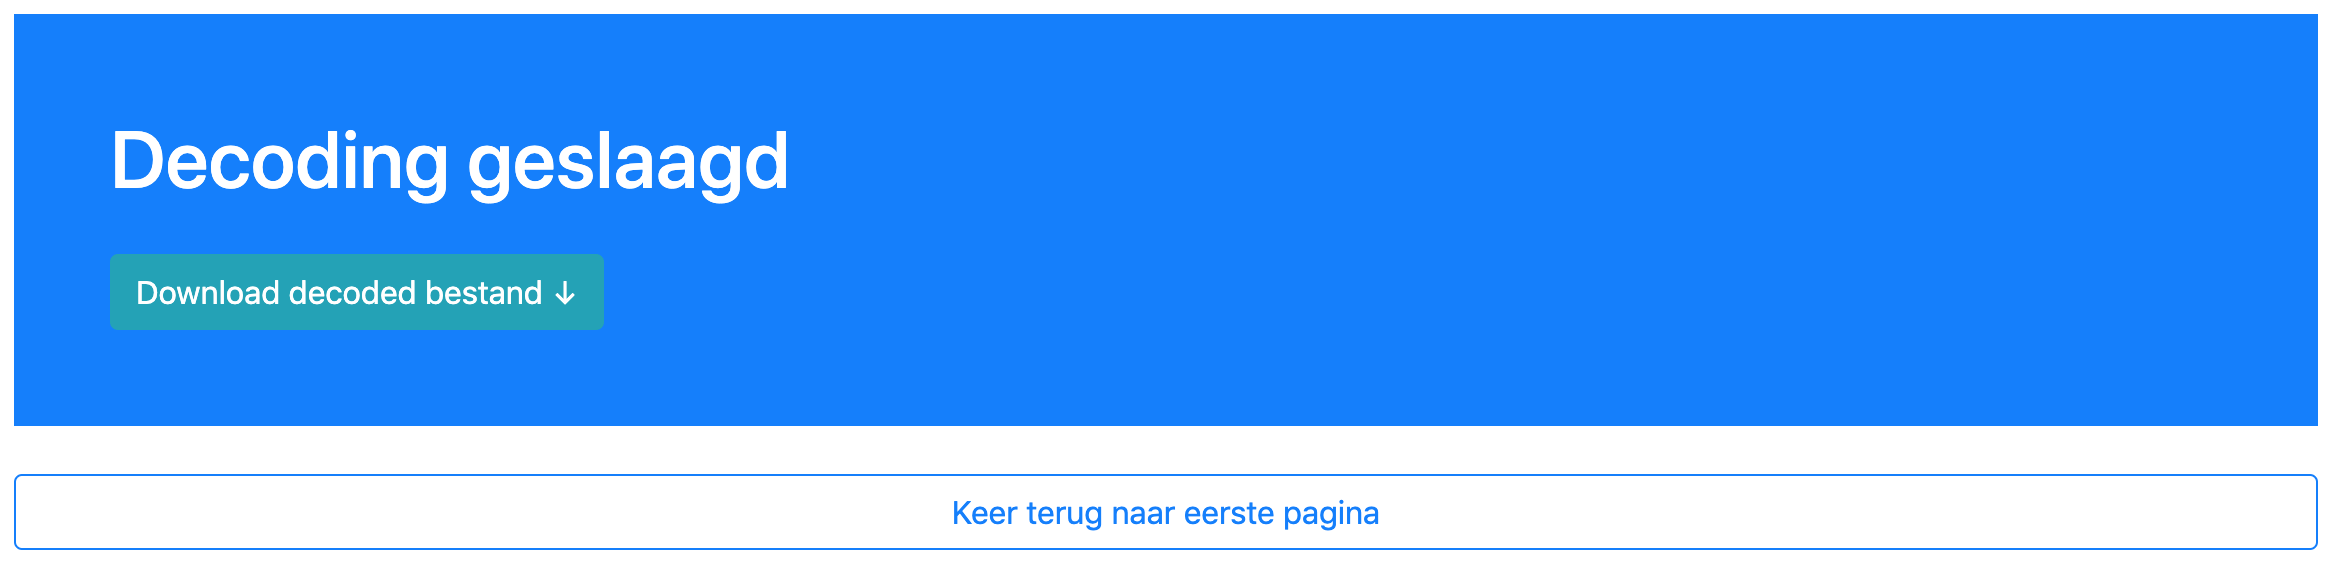
\includegraphics[width=\linewidth]{img/bijlages/compressietool/decoded.png}}
	\caption{Scherm verkregen door een bestand te decoderen \gls{afbeeldingsevaluatietool}.}
	\label{fig:bijlages-screenshot-datacompressietool-decoded}
\end{figure}
\FloatBarrier


\section{Screenshots afbeeldingsevaluatietool}
\label{sec:bijlages-screenshot-afbeeldingsevaluatietool}

De \gls{afbeeldingsevaluatietool} is raadpleegbaar via de website van Lennert Bontinck\urlcite{evaluatietool}. De code is te vinden op de \gls{github} repository van deze bachelorproef\urlcite{githubbachelorproef}.

\FloatBarrier
\begin{figure}[h!]
	\fbox{
\includegraphics[width=\linewidth]{img/bijlages/afbeeldingsevaluatietool/setup.png}}
	\caption{Setup scherm van de \gls{afbeeldingsevaluatietool}.}
	\label{fig:bijlages-screenshot-afbeeldingsevaluatietool-setup}
\end{figure}
\FloatBarrier

\FloatBarrier
\begin{figure}[h!]
	\fbox{
\includegraphics[width=\linewidth]{img/bijlages/afbeeldingsevaluatietool/welkom.png}}
	\caption{Verwelkomingsscherm van de \gls{afbeeldingsevaluatietool}.}
	\label{fig:bijlages-screenshot-afbeeldingsevaluatietool-welkom}
\end{figure}
\FloatBarrier

\FloatBarrier
\begin{figure}[h!]
	\fbox{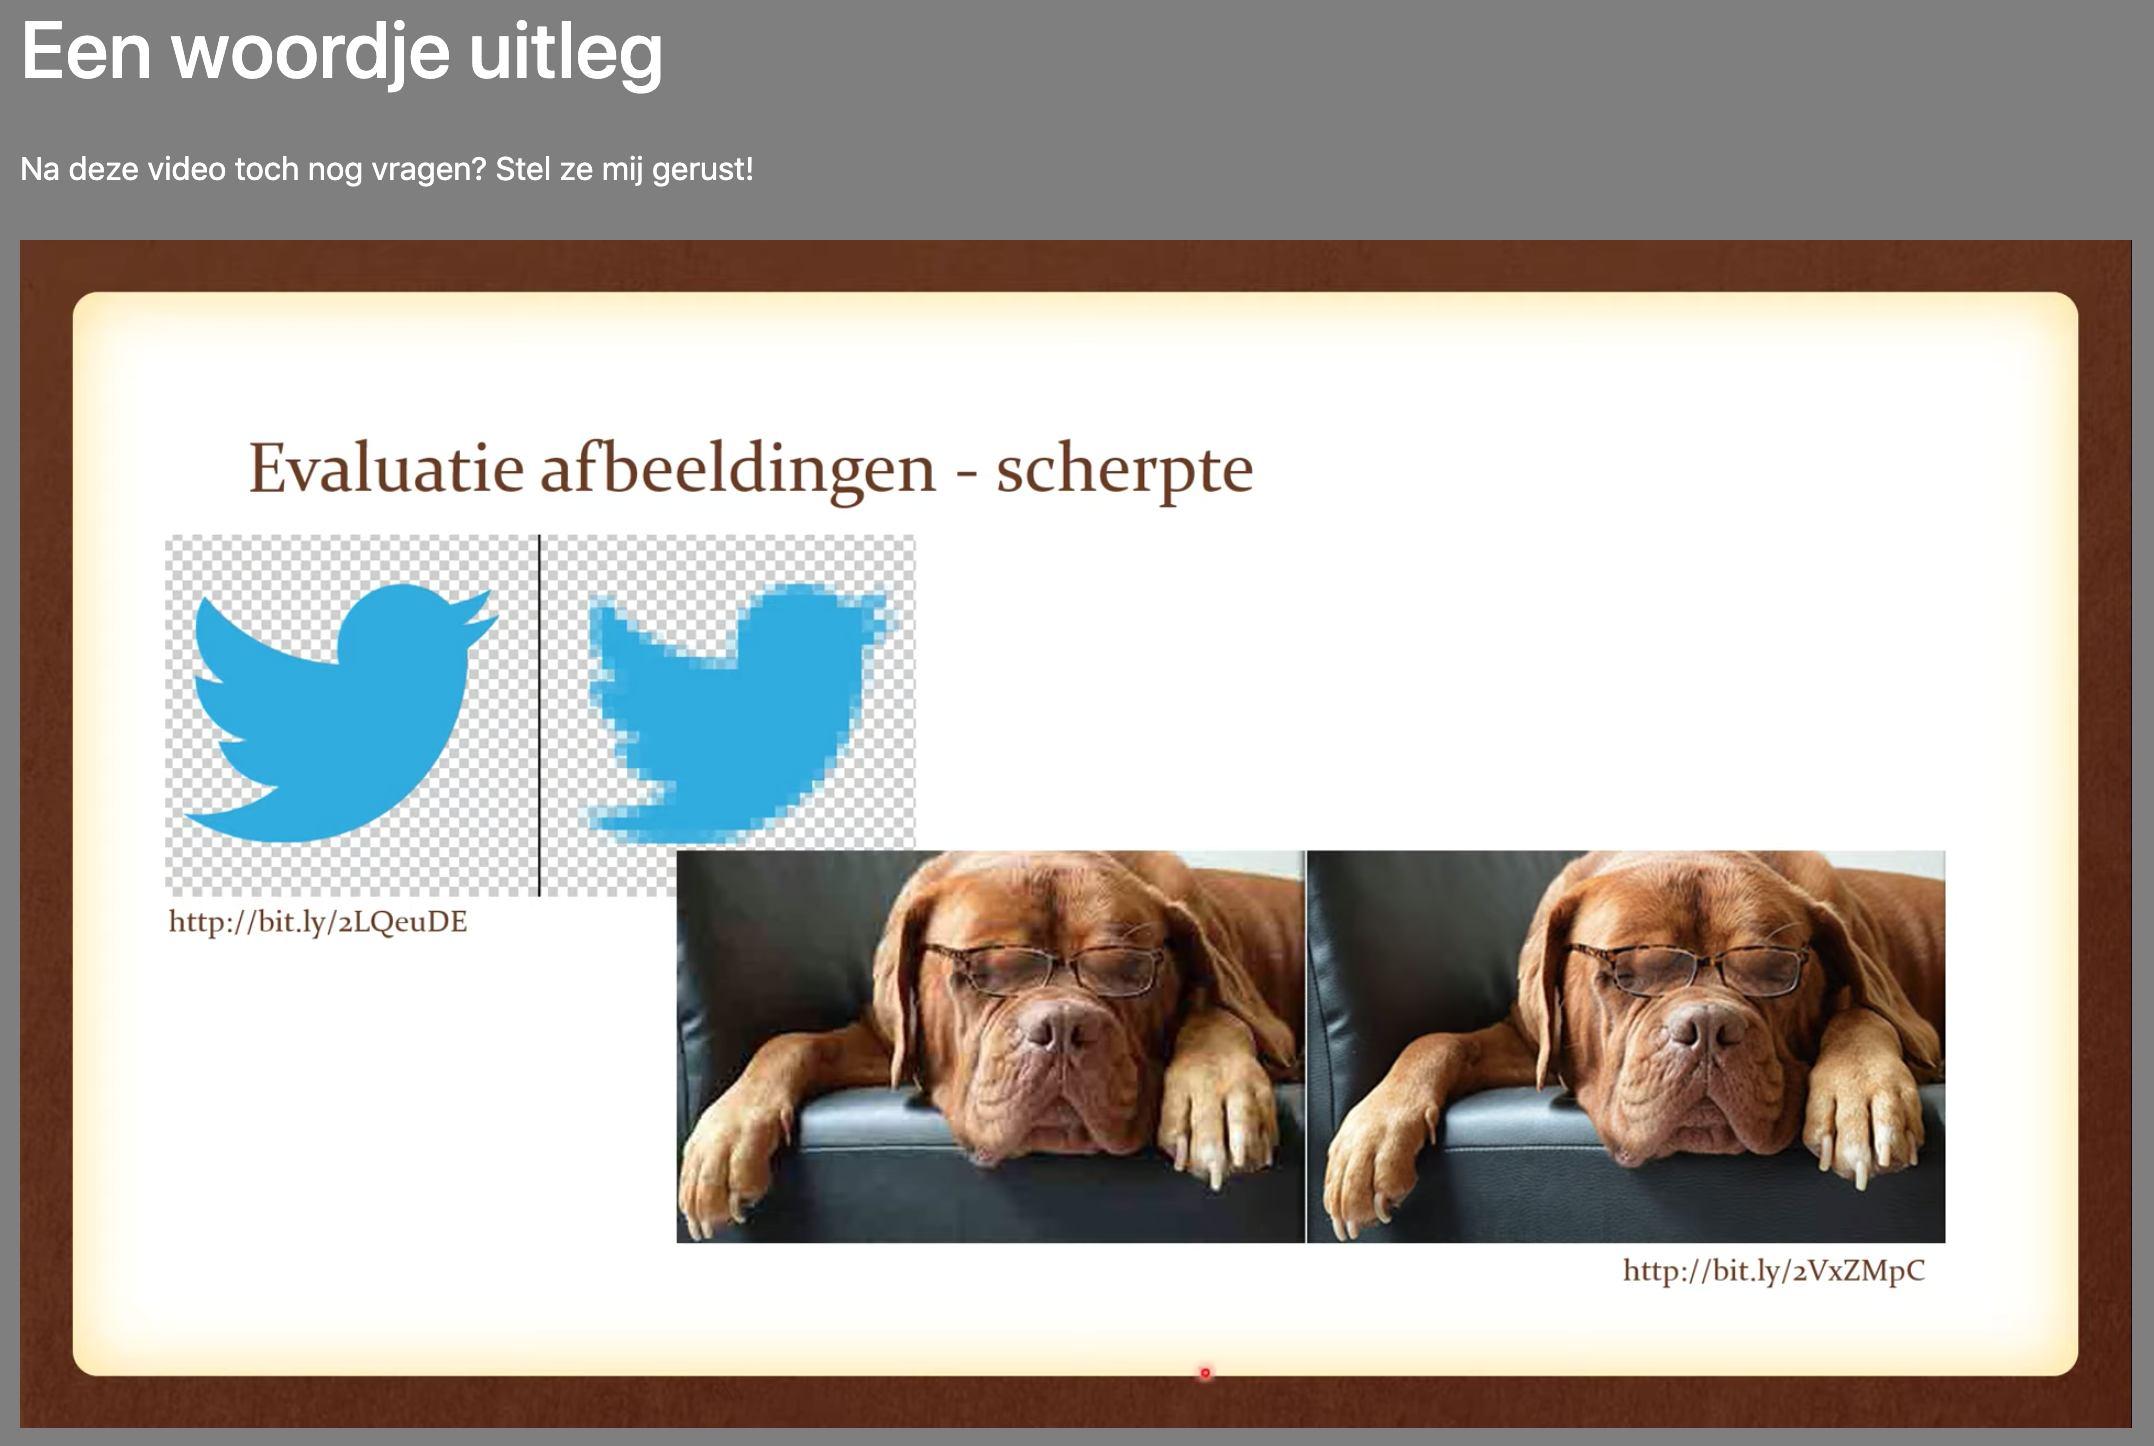
\includegraphics[width=\linewidth]{img/bijlages/afbeeldingsevaluatietool/video.png}}
	\caption{Introductievideo met uitleg van de \gls{afbeeldingsevaluatietool}.}
	\label{fig:bijlages-screenshot-afbeeldingsevaluatietool-video}
\end{figure}
\FloatBarrier

\FloatBarrier
\begin{figure}[h!]
	\fbox{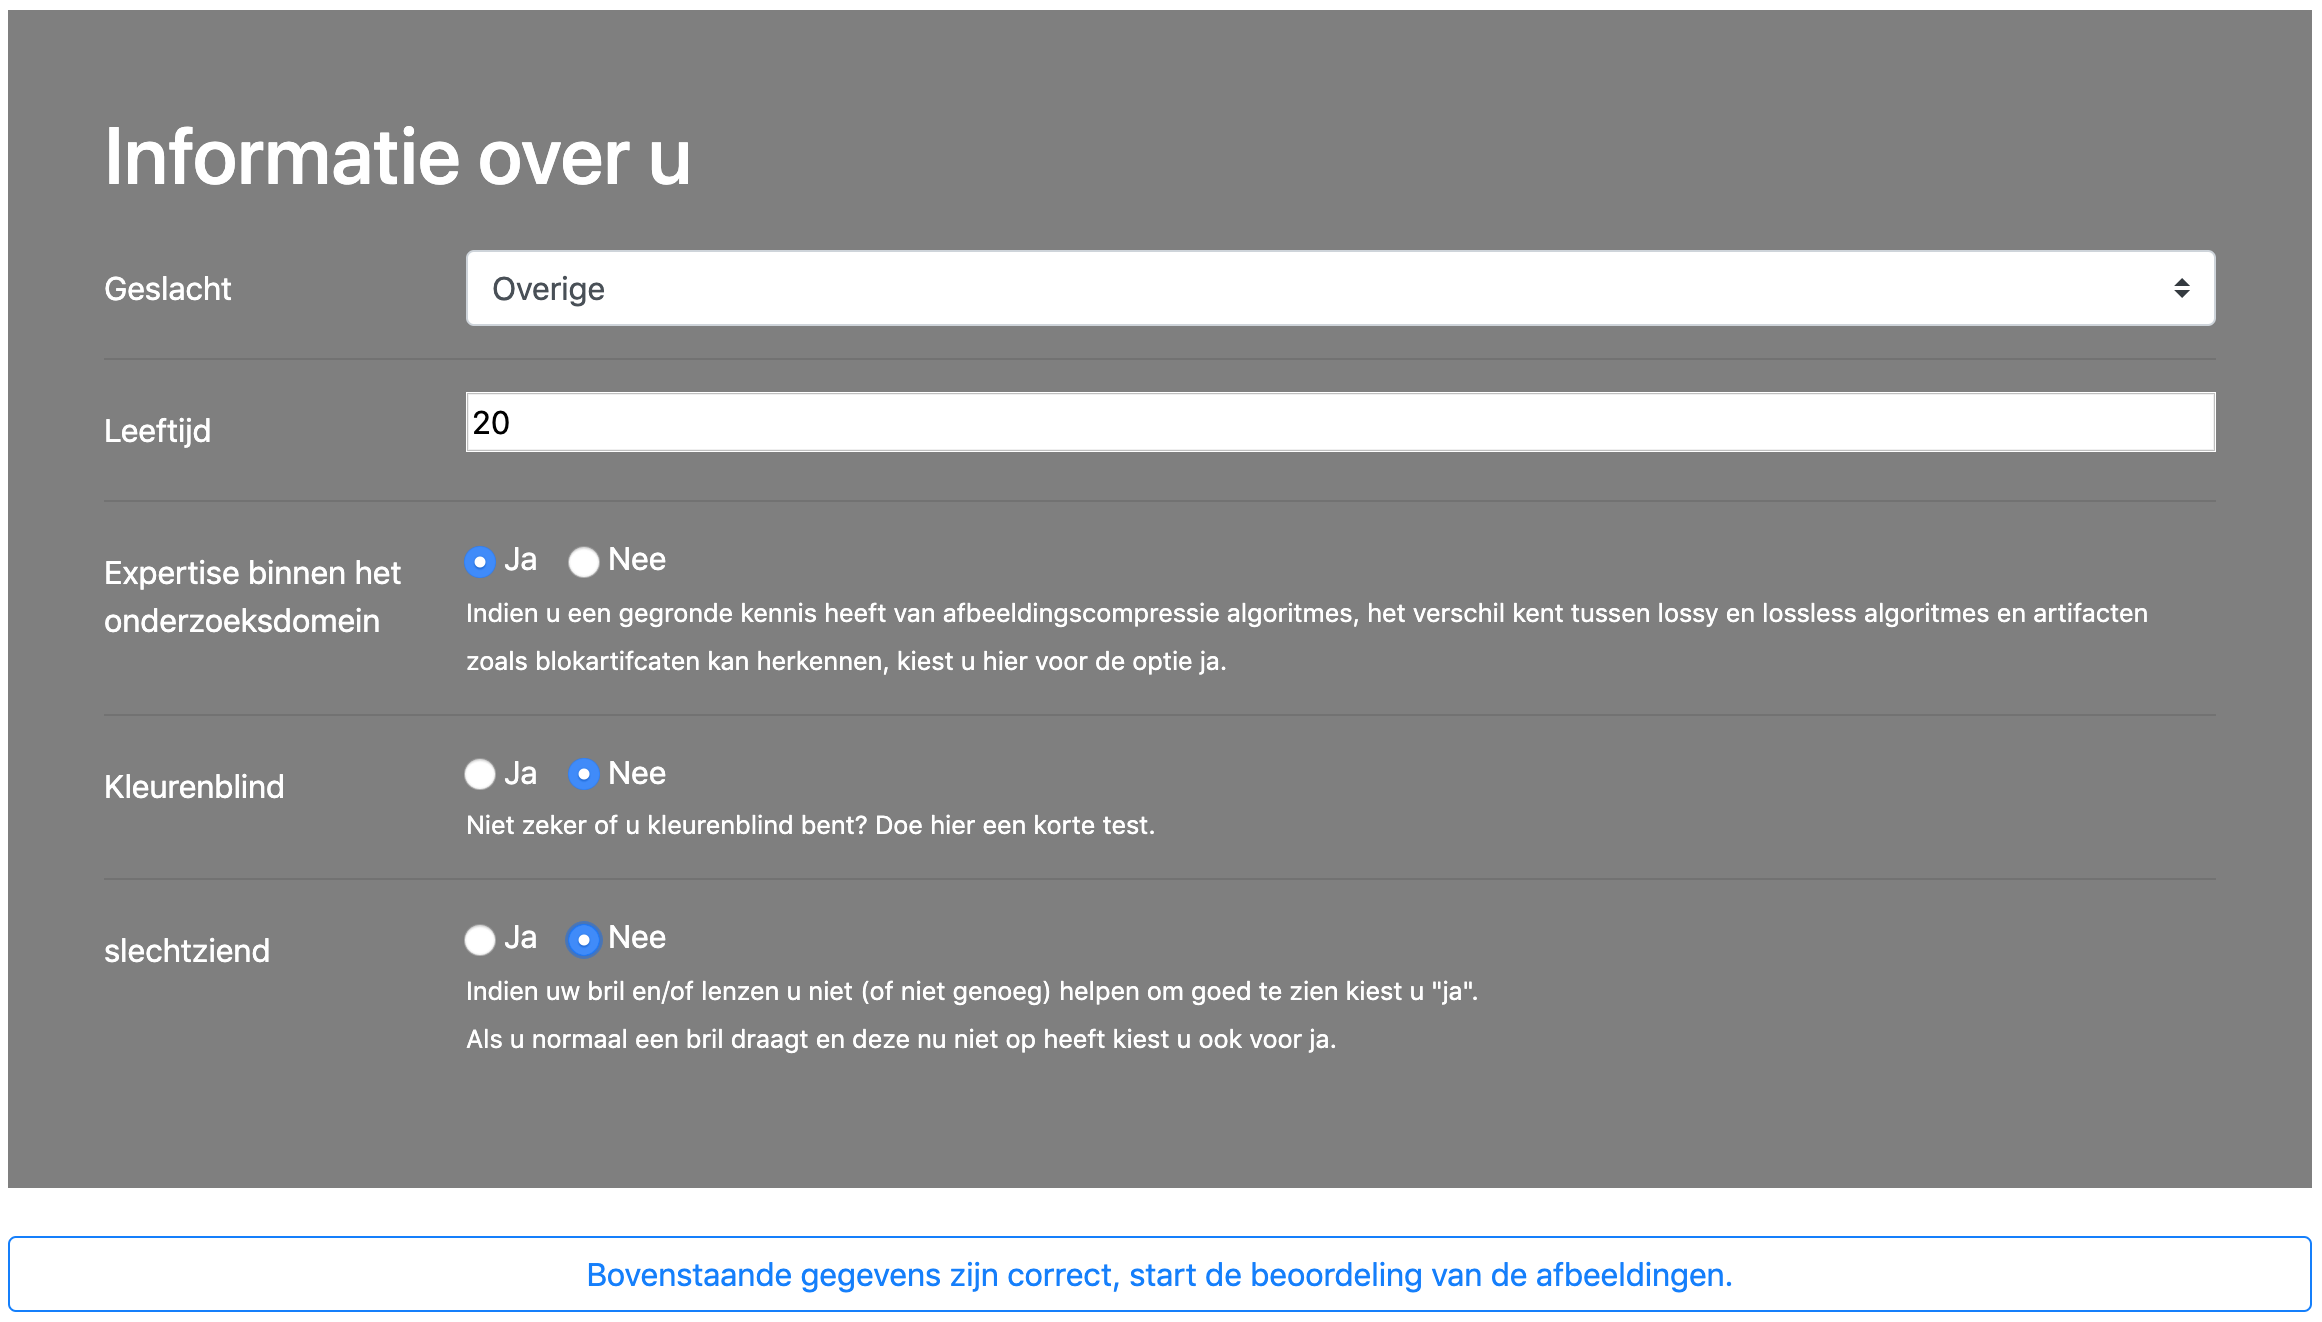
\includegraphics[width=\linewidth]{img/bijlages/afbeeldingsevaluatietool/over-u.png}}
	\caption{Informatie over de deelnemer in de \gls{afbeeldingsevaluatietool}.}
	\label{fig:bijlages-screenshot-afbeeldingsevaluatietool-over-u}
\end{figure}
\FloatBarrier

\FloatBarrier
\begin{figure}[h!]
	\fbox{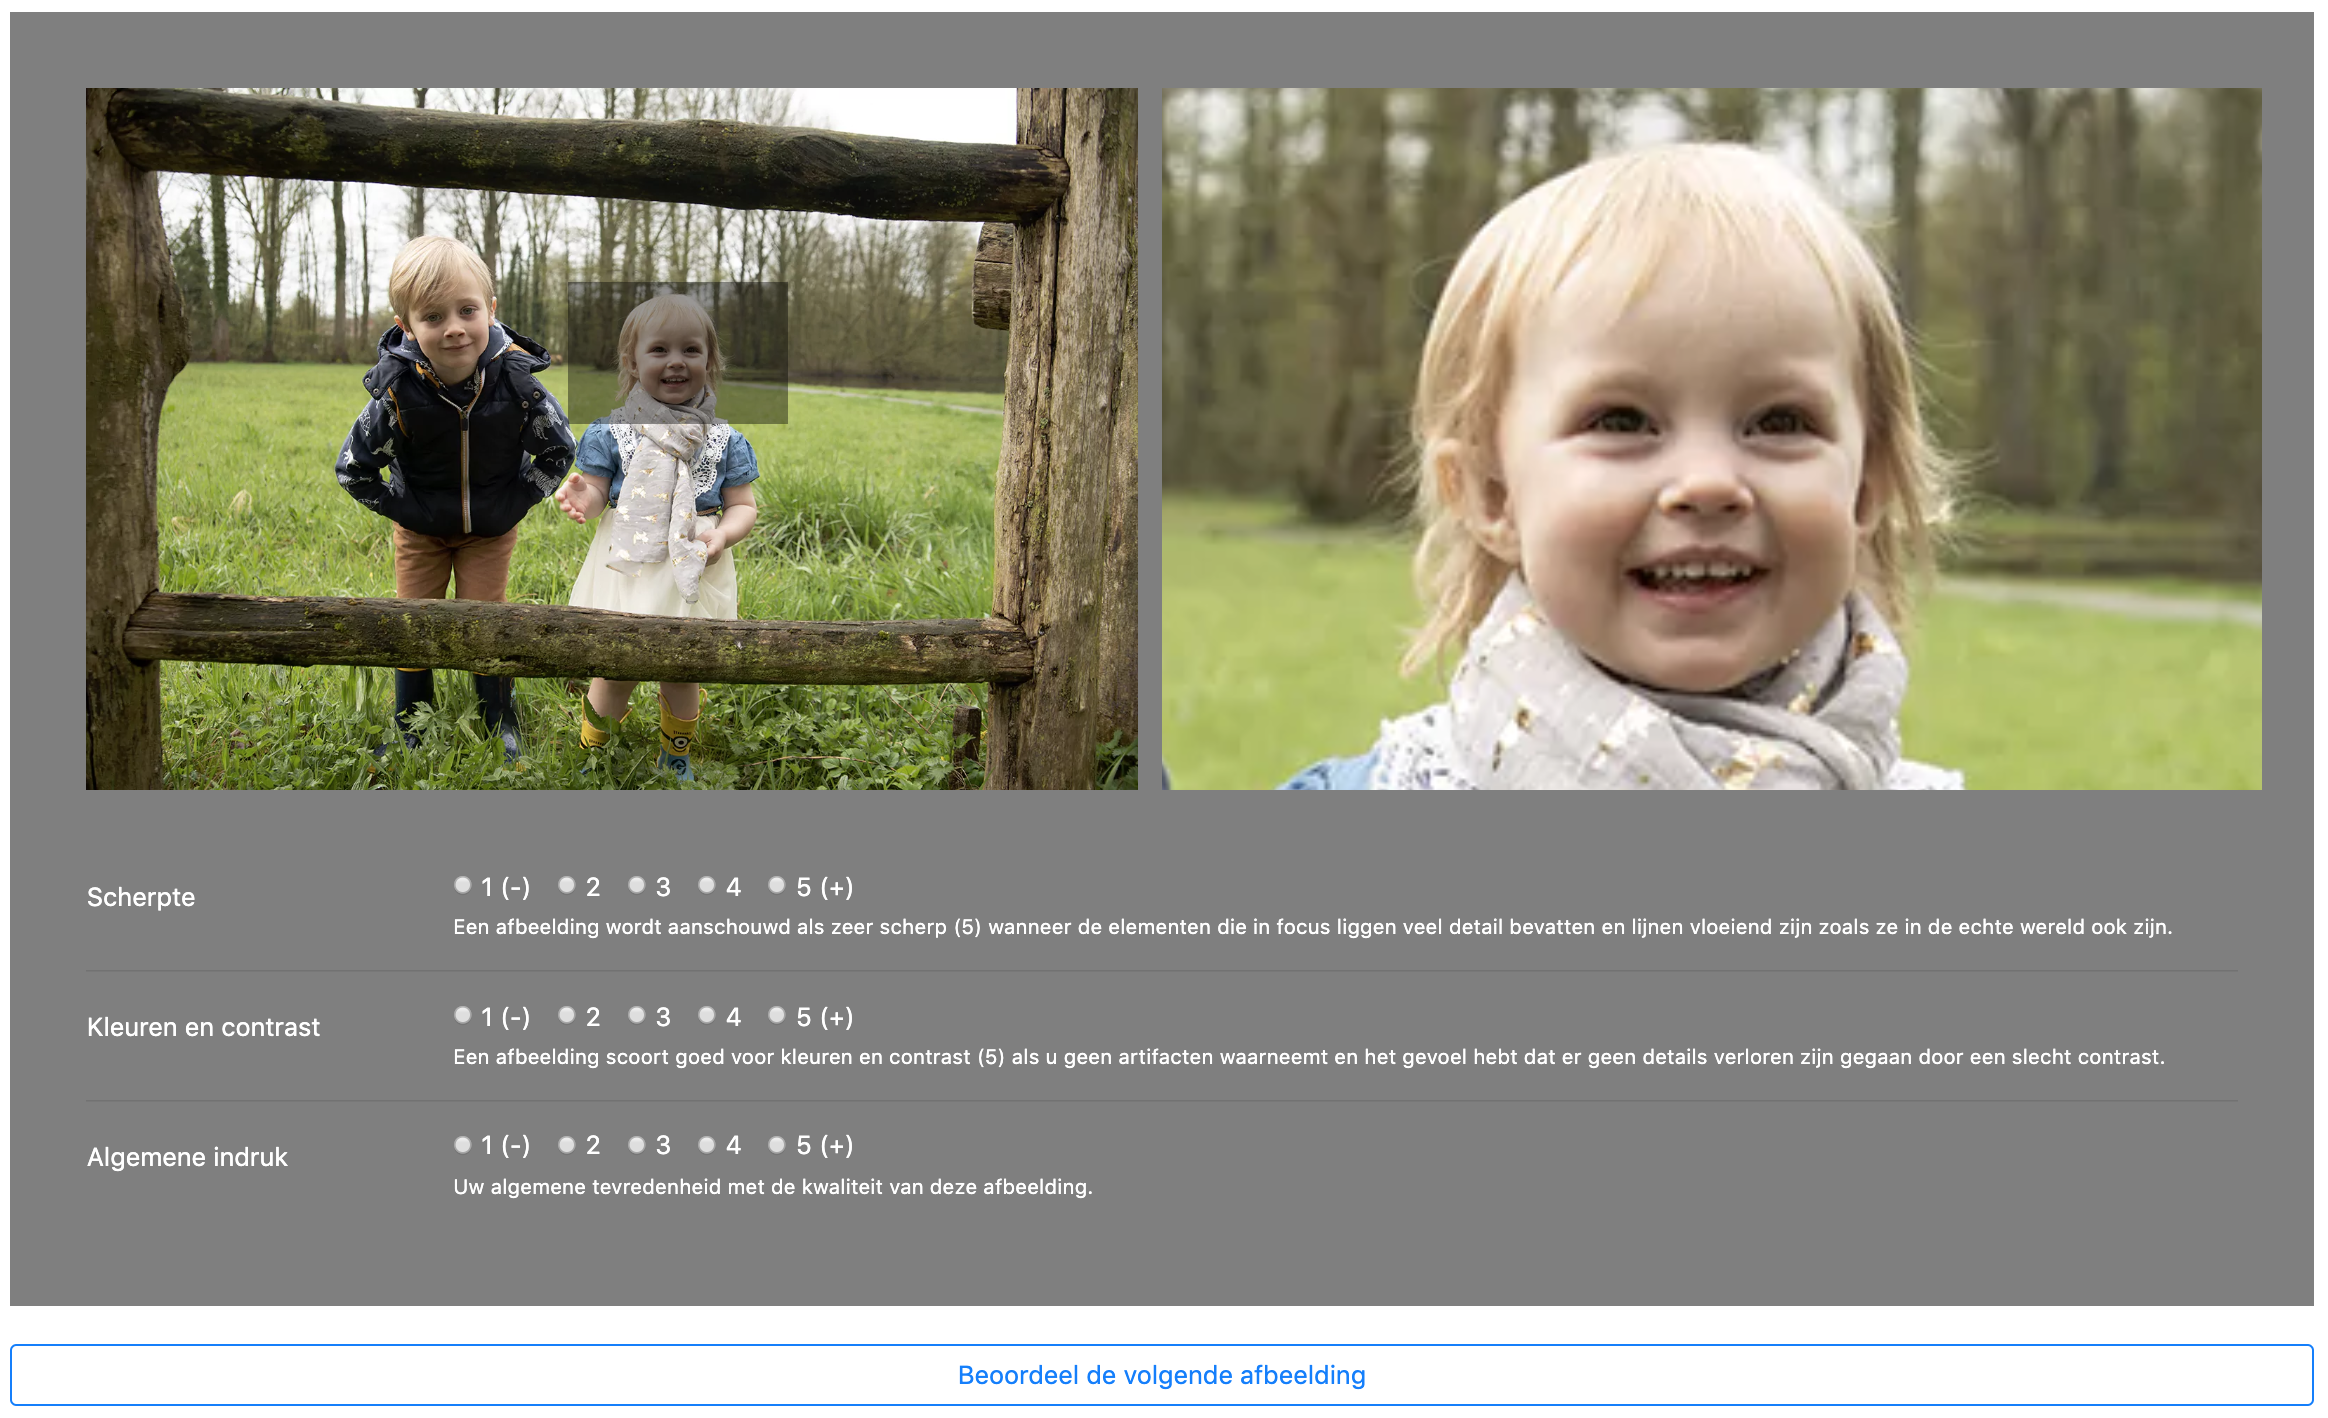
\includegraphics[width=\linewidth]{img/bijlages/afbeeldingsevaluatietool/evaluatie.png}}
	\caption{Afbeelding beoordelen in de \gls{afbeeldingsevaluatietool} met 5x zoom mogelijkheid.}
	\label{fig:bijlages-screenshot-afbeeldingsevaluatietool-evalutie}
\end{figure}
\FloatBarrier

\FloatBarrier
\begin{figure}[h!]
	\fbox{
\includegraphics[width=\linewidth]{img/bijlages/afbeeldingsevaluatietool/export.png}}
	\caption{Het scherm waar de resultaat gedownload kunnen worden.}
	\label{fig:bijlages-screenshot-afbeeldingsevaluatietool-export}
\end{figure}
\FloatBarrier

\section{Extra documenten onderzoek}
\label{sec:bijlages-onderzoek}

\FloatBarrier
\begin{figure}[h!]
	\centering
	\fbox{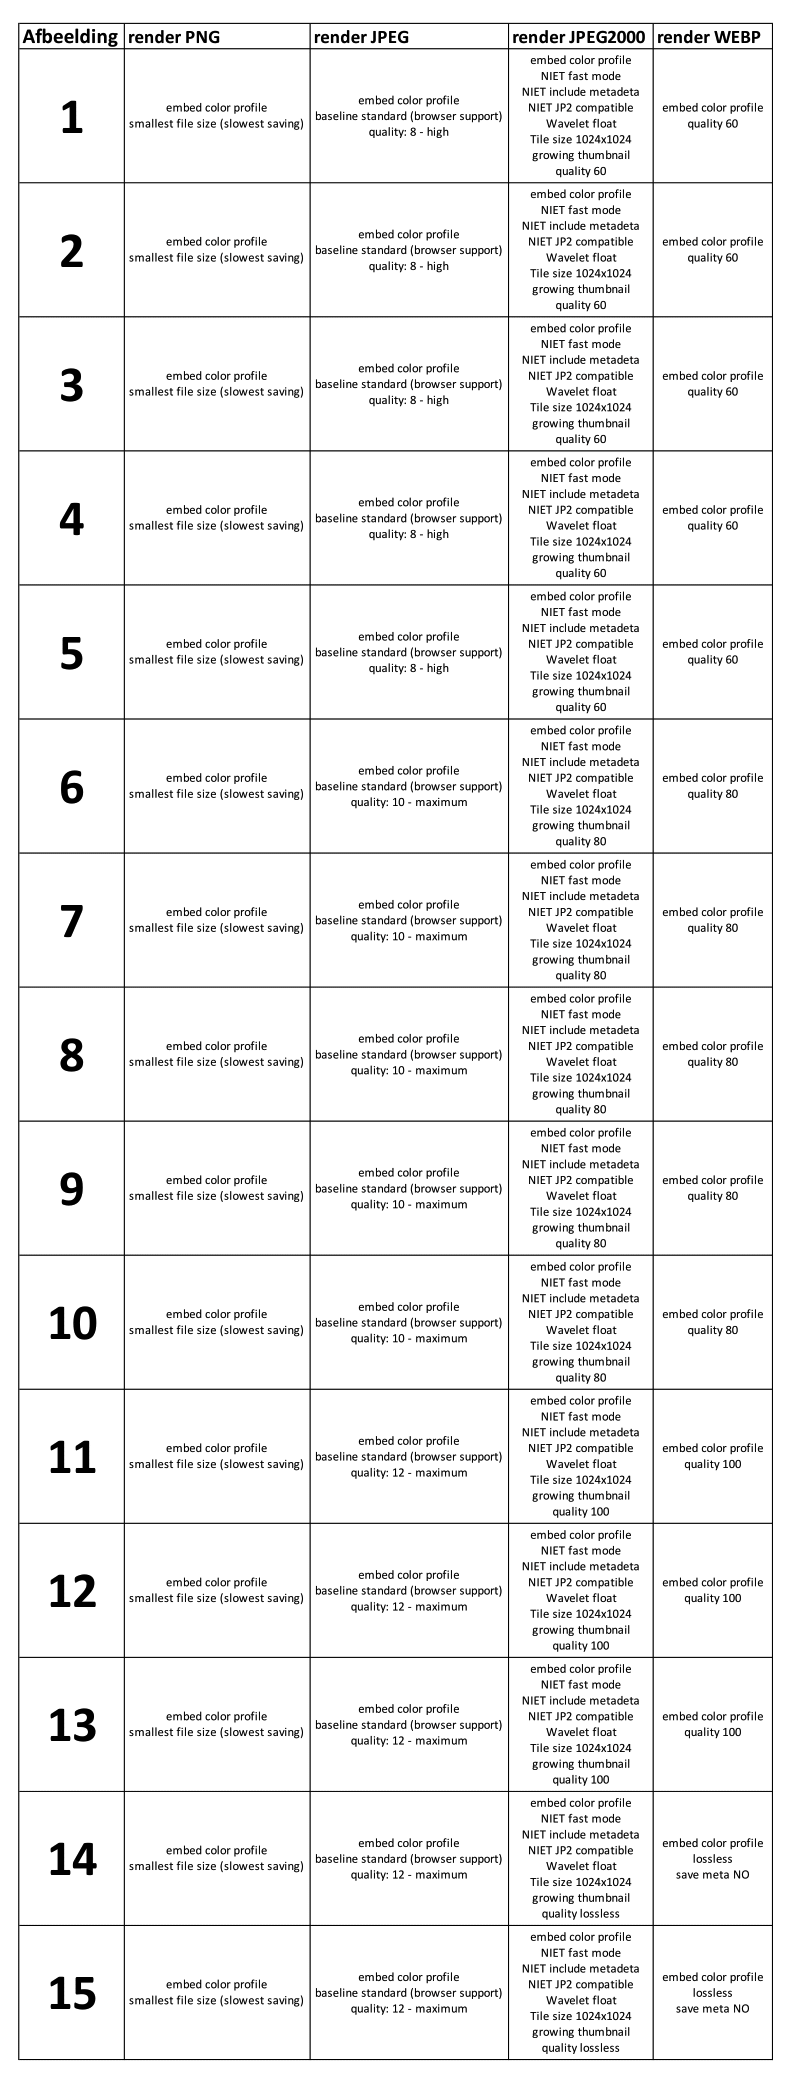
\includegraphics[width=0.5\linewidth]{img/bijlages/onderzoek/renderopties.png}}
	\caption{De renderopties ingesteld in \gls{ps} voor alle vijftien afbeeldingen en vier \glspl{afbeeldingsformaat}.}
	\label{fig:bijlages-onderzoek-render}
\end{figure}
\FloatBarrier

\FloatBarrier
\begin{figure}[h!]
	\centering
	\fbox{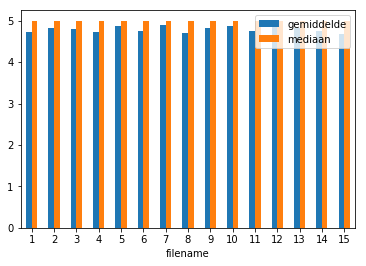
\includegraphics[width=0.5\linewidth]{img/bijlages/onderzoek/resultaat/lossless/png-gem-med.png}}
	\caption{Het gemiddelde en de mediaan voor het kenmerk 'algemene indruk' van afbeeldingen met het \gls{lossless} \gls{png} afbeeldingsformaat.}
	\label{fig:bijlages-onderzoek-resultaten-png-gem-med}
\end{figure}
\FloatBarrier

\FloatBarrier
\begin{figure}[h!]
	\centering
	\fbox{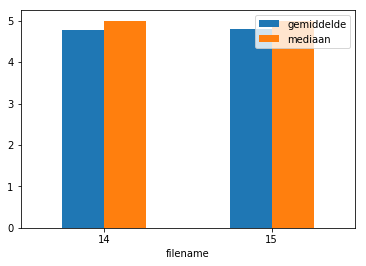
\includegraphics[width=0.5\linewidth]{img/bijlages/onderzoek/resultaat/lossless/lossless-webp-gem-med.png}}
	\caption{Het gemiddelde en de mediaan voor het kenmerk 'algemene indruk' van afbeeldingen met het \gls{lossless} \gls{webp} afbeeldingsformaat.}
	\label{fig:bijlages-onderzoek-resultaten-lossless-webp-gem-med}
\end{figure}
\FloatBarrier

\FloatBarrier
\begin{figure}[h!]
	\centering
	\fbox{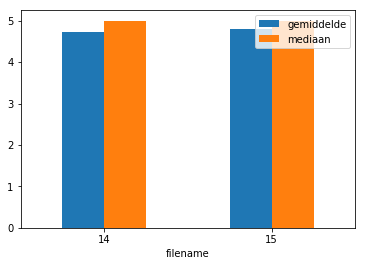
\includegraphics[width=0.5\linewidth]{img/bijlages/onderzoek/resultaat/lossless/lossless-jpeg2000-gem-med.png}}
	\caption{Het gemiddelde en de mediaan voor het kenmerk 'algemene indruk' van afbeeldingen met het \gls{lossless} \gls{jpeg2000} afbeeldingsformaat.}
	\label{fig:bijlages-onderzoek-resultaten-lossless-jpeg2000-gem-med}
\end{figure}
\FloatBarrier

\FloatBarrier
\begin{figure}[h!]
	\centering
	\fbox{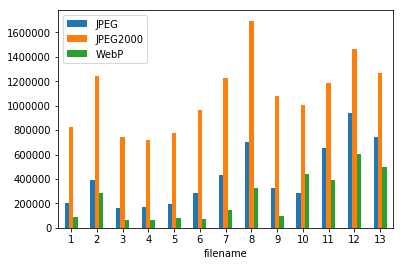
\includegraphics[width=0.5\linewidth]{img/bijlages/onderzoek/resultaat/lossy/lossy_sizes.png}}
	\caption{De bestandsgrootte in \glspl{bit} voor de afbeeldingen dat \gls{lossy} gecomprimeerd zijn door zowel \gls{jpeg}, \gls{jpeg2000} en \gls{webp}.}
	\label{fig:onderzoek-resultaten-lossy-sizes}
\end{figure}
\FloatBarrier

\FloatBarrier
\begin{figure}[h!]
	\centering
	\fbox{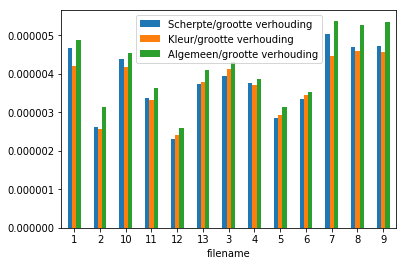
\includegraphics[width=0.5\linewidth]{img/bijlages/onderzoek/resultaat/lossy/lossy_rating_ratio_jpf.png}}
	\caption{Verhouding van de gemiddelde score ten opzichte van de bestandsgrootte voor \gls{jpf}.}
	\label{fig:onderzoek-resultaten-lossy-ratio-jpf}
\end{figure}
\FloatBarrier

\FloatBarrier
\begin{figure}[h!]
	\centering
	\fbox{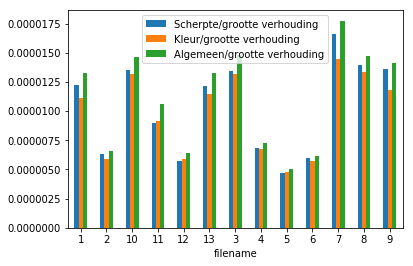
\includegraphics[width=0.5\linewidth]{img/bijlages/onderzoek/resultaat/lossy/lossy_rating_ratio_jpg.png}}
	\caption{Verhouding van de gemiddelde score ten opzichte van de bestandsgrootte voor \gls{jpeg}.}
	\label{fig:onderzoek-resultaten-lossy-ratio-jpg}
\end{figure}
\FloatBarrier

\FloatBarrier
\begin{figure}[h!]
	\centering
	\fbox{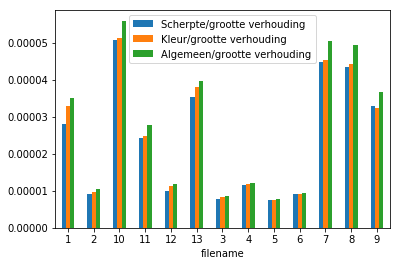
\includegraphics[width=0.5\linewidth]{img/bijlages/onderzoek/resultaat/lossy/lossy_rating_ratio_webp.png}}
	\caption{Verhouding van de gemiddelde score ten opzichte van de bestandsgrootte voor \gls{webp}.}
	\label{fig:onderzoek-resultaten-lossy-ratio-webp}
\end{figure}
\FloatBarrier